% The package's structure (README, docs index, report), laid out like the OlmoEarth architecture figure: real imagery
% on the left (Sentinel-2 of scene okavango_80, 1.28 km at 10 m/px, with the frozen-encoder water map, its confidence
% and WorldCover as a second map, from rasters/ as make_rasters.py writes them), the structure on the right (chevrons
% for operations, squares for windows, pink boxes for what the user gets), bold captions under each half. 1.12.0: the
% which-map row names the better map by an exact test (1.10.0), and a row for the per-class audit (1.11.0).
% Build: pdflatex architecture.tex; export: osascript -l JavaScript pdf2png.js architecture.pdf ../architecture.png 3600
\documentclass[tikz,border=3mm]{standalone}
\usepackage[T1]{fontenc}
\usepackage{helvet}
\renewcommand{\familydefault}{\sfdefault}
\usepackage{amssymb}
\usepackage{graphicx}
\pagecolor{white}
\usetikzlibrary{positioning,arrows.meta,shadows,shapes.geometric,shapes.symbols,calc,fit,backgrounds}
\definecolor{ink}{HTML}{1F2937}\definecolor{muted}{HTML}{6B7280}
\definecolor{s2}{HTML}{E2559B}\definecolor{mapo}{HTML}{F59E0B}\definecolor{pinkout}{HTML}{E94E9B}
\definecolor{teal}{HTML}{0F766E}\definecolor{amber}{HTML}{D97706}\definecolor{violet}{HTML}{6D28D9}
\definecolor{red}{HTML}{DC2626}\definecolor{green}{HTML}{16A34A}\definecolor{sky}{HTML}{BFDBFE}
\hyphenpenalty=10000 \exhyphenpenalty=10000
\tikzset{
  >=Stealth, font=\normalsize,
  flow/.style={->, line width=0.8pt, draw=ink},
  panel/.style={draw=ink!25, dashed, fill=ink!2, line width=0.6pt},
  ptitle/.style={font=\large\bfseries, text=ink, inner sep=1pt},
  caption/.style={font=\Large\bfseries, text=ink, inner sep=1pt},
  img/.style={inner sep=0pt, line width=1.3pt, drop shadow={shadow xshift=1.0mm, shadow yshift=-1.0mm, opacity=0.25}},
  thumb/.style={img, draw=mapo, line width=1.4pt},
  tlabel/.style={font=\small, text=ink, inner sep=1pt},
  op/.style={signal, signal to=east, signal from=west, draw=ink, fill=#1, line width=0.8pt,
             minimum height=10.5mm, text width=1.9cm, align=center, font=\footnotesize, inner xsep=1pt},
  op/.default=white,
  result/.style={draw=ink, dashed, fill=pinkout, text=white, rounded corners=2pt, line width=0.8pt, minimum height=11.5mm,
              text width=3.9cm, align=center, font=\small, drop shadow={shadow xshift=0.6mm, shadow yshift=-0.6mm, opacity=0.2}},
  tok/.style={draw=ink!70, line width=0.5pt, minimum size=3.9mm, inner sep=0pt},
  note/.style={font=\footnotesize, text=muted, align=center, inner sep=1pt},
  part/.style={draw=ink, line width=0.8pt, drop shadow={shadow xshift=0.8mm, shadow yshift=-0.8mm, opacity=0.25}},
  lane/.style={draw=ink!25, dashed, rounded corners=4pt, line width=0.6pt},
  lanetitle/.style={font=\small\bfseries, text=ink, inner sep=1pt, anchor=north west},
}
\begin{document}
\begin{tikzpicture}
  % column positions (cm); a chevron is 2.55 wide and 0.9 high, a window square 0.39
  \def\bus{14.05}\def\laneL{14.25}\def\laneR{28.5}\def\colA{15.95}\def\tokx{17.95}\def\colB{22.35}\def\outx{24.05}

  % ======================================================================= your data and model
  % the left half and its link to the bus, lowered to sit level with the taller right half
  \begin{scope}[yshift=-1.3cm]
  \node[ptitle] at (2.25,8.55) {Satellite observations};
  \begin{scope}[on background layer] \draw[panel] (0.15,2.45) rectangle (4.35,8.15); \end{scope}
  \node[img, draw=s2!55] (bs) at (2.75,5.84) {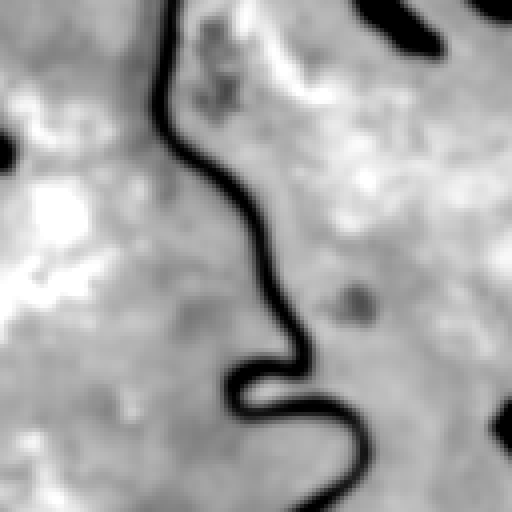
\includegraphics[width=2.55cm]{rasters/scene_b11.png}};
  \node[img, draw=s2!75] (bn) at (2.47,5.56) {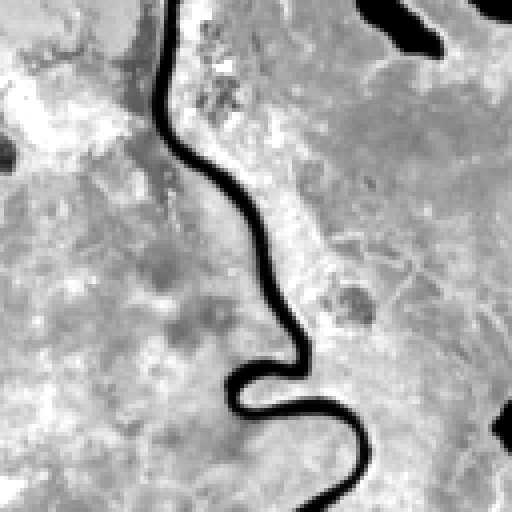
\includegraphics[width=2.55cm]{rasters/scene_b08.png}};
  \node[img, draw=s2] (br) at (2.19,5.28) {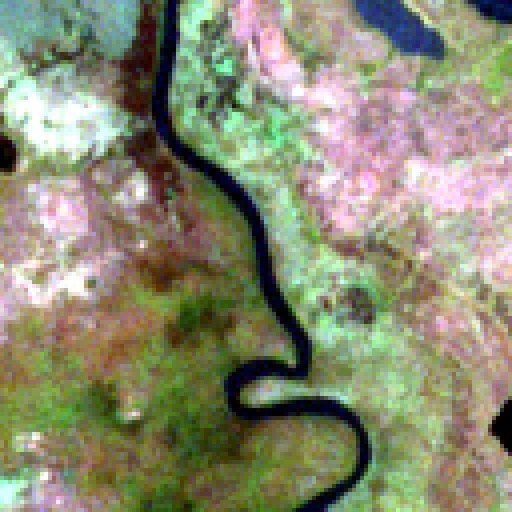
\includegraphics[width=2.55cm]{rasters/scene_rgb.png}};
  \foreach \n/\t in {bs/SWIR, bn/NIR, br/{RGB, 10\,m/px}} {\node[font=\scriptsize\bfseries, text=white, fill=ink, fill opacity=0.55, text opacity=1, inner sep=1.5pt, anchor=north east] at ($(\n.north east)+(-0.04,-0.04)$) {\t};}
  \node[font=\normalsize\bfseries, rotate=90, text=ink] at (0.5,5.28) {Sentinel-2};
  \draw[ink!60, |-|, line width=0.5pt] ($(br.south west)+(0,-0.2)$) -- ($(br.south east)+(0,-0.2)$)
        node[midway, below, font=\scriptsize, text=muted] {1.28\,km};

  % the model: encoder narrows, decoder widens, names inside
  \draw[flow] (4.42,5.19) -- (4.7,5.19);
  \draw[part, fill=ink!10] (4.78,3.85) -- (4.78,6.55) -- (5.55,5.85) -- (5.55,4.55) -- cycle;
  \draw[part, fill=ink!10] (5.72,4.55) -- (5.72,5.85) -- (6.49,6.55) -- (6.49,3.85) -- cycle;
  \node[font=\footnotesize\bfseries, text=ink, rotate=90] at (5.12,5.2) {Encoder};
  \node[font=\footnotesize\bfseries, text=ink, rotate=90] at (6.15,5.2) {Decoder};
  \node[note] at (5.63,3.35) {any EO model};
  \draw[flow] (6.55,5.19) -- (6.85,5.19);

  % model outputs: what the package reads, the class map and the confidence
  \node[ptitle] at (8.4,8.55) {Model outputs};
  \begin{scope}[on background layer] \draw[panel] (6.95,2.45) rectangle (9.85,8.15); \end{scope}
  \node[tlabel] at (8.35,7.56) {Class map};
  \node[thumb] (pred) at (8.35,6.49) {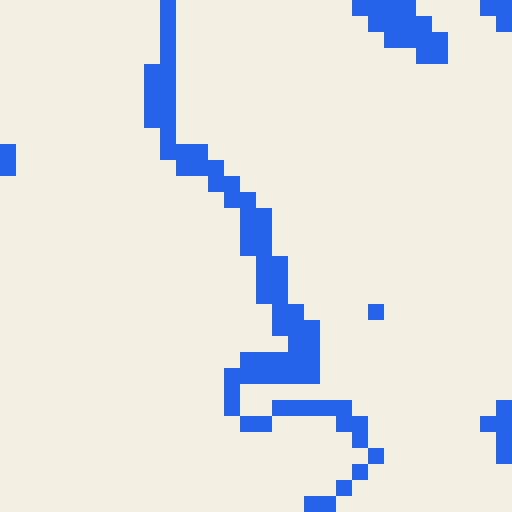
\includegraphics[width=1.75cm]{rasters/scene_pred.png}};
  \node[tlabel] at (8.35,4.96) {Confidence};
  \node[thumb] (conf) at (8.35,3.89) {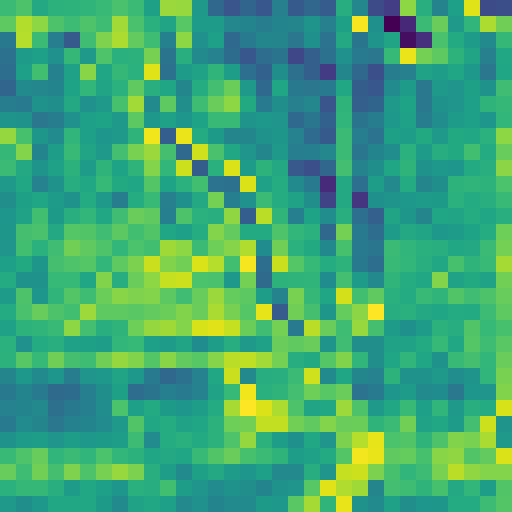
\includegraphics[width=1.75cm]{rasters/scene_conf.png}};

  % ======================================================================= olmoearth-inferenceX
  \node[op=sky] (pool) at (11.3,5.19) {Pool to\\ windows};
  \draw[flow] (9.92,5.19) -- (pool.west);
  % window squares, centred on the flow line
  \foreach \s [count=\i] in {90,35,80,20,95,60} {\node[tok, fill=teal!\s!white] (w\i) at (13.35,{5.19+0.42*(3.5-\i)}) {};}
  \draw[flow] (pool.east) -- (13.13,5.19);
  \node[note, anchor=north] at (13.22,4.0) {class +\\ confidence};
  \draw[line width=0.9pt, draw=ink] (13.57,5.19) -- (\bus,5.19);
  \end{scope}
  \node[caption] at (5.0,-0.45) {Your data and model};
  \draw[line width=0.9pt, draw=ink] (\bus,8.0) -- (\bus,1.05);

  % ---- without reference labels
  \draw[lane] (\laneL,6.15) rectangle (\laneR,9.1);
  \node[lanetitle] at (\laneL+0.1,9.05) {Without reference labels};
  \node[op] (rank) at (\colA,8.0) {Rank by\\ confidence};
  \draw[flow] (\bus,8.0) -- (rank.west);
  \foreach \s [count=\i] in {20,32,45,60,74,86,94} {\node[tok, fill=teal!\s!white] (r\i) at ({\tokx+0.42*(\i-1)},8.0) {};}
  \draw[draw=pinkout, line width=1.3pt] ($(r1.south west)+(-0.05,-0.05)$) rectangle ($(r2.north east)+(0.05,0.05)$);
  \node[note, anchor=south west] at ($(r1.north west)+(-0.05,0.1)$) {lowest confidence first};
  \draw[flow] (rank.east) -- (r1.west);
  \node[result, anchor=west] (o1) at (\outx,8.0) {\textbf{Review set}\\ windows to inspect first};
  \draw[flow] (r7.east) -- (o1.west);
  \node[op] (cmp) at (\colA,6.75) {Compare\\ A and B};
  \draw[flow] (\bus,6.75) -- (cmp.west);
  \foreach \d [count=\i] in {0,1,0,1,1,0,0} {\node[tok, fill=\ifcase\d white\or red!35\fi] (c\i) at ({\tokx+0.42*(\i-1)},6.75) {};}
  \draw[flow] (cmp.east) -- (c1.west);
  \node[result, anchor=west] (o2) at (\outx,6.75) {\textbf{Disagreement map}\\ rate, location, boundaries};
  \draw[flow] (c7.east) -- (o2.west);

  % ---- with a labelled sample
  \draw[lane] (\laneL,0.0) rectangle (\laneR,5.95);
  \node[lanetitle] at (\laneL+0.1,5.9) {With a labelled sample};
  % the differing windows, sampled and labelled: which map is right
  \foreach \m [count=\i] in {1,1,0,1,1} {
     \node[tok, fill=red!15, draw=violet, line width=0.8pt] (p\i) at ({\tokx+0.42*(\i-1)},4.85) {};
     \node[font=\scriptsize\bfseries, inner sep=0pt] at (p\i) {\ifcase\m B\or A\fi};}
  \draw[flow] (c4.south) -- (p4.north);
  \node[note, anchor=west] at ($(c4.south)!0.62!(p4.north)+(0.15,0)$) {sample of the differing windows};
  \node[note, anchor=north west, text=violet] at ($(p1.south west)+(-0.05,-0.1)$) {correct map: A or B};
  \node[op] (diff) at (\colB,4.85) {Exact test\\ and interval};
  \draw[flow] (p5.east) -- (diff.west);
  \node[result, anchor=west] (o5) at (\outx,4.85) {\textbf{Which map is better}\\ and A $-$ B, 95\% interval};
  \draw[flow] (diff.east) -- (o5.west);
  % a random sample of all windows, labelled: the error rate and the certified zone
  \node[op] (samp) at (\colA,3.55) {Random\\ sample};
  \draw[flow] (\bus,3.55) -- (samp.west);
  \foreach \m [count=\i] in {1,1,0,1,2,1} {
     \node[tok, fill=white, draw=violet, line width=0.8pt] (q\i) at ({\tokx+0.42*(\i-1)},3.55) {};
     \ifcase\m \node[text=red, font=\scriptsize\bfseries, inner sep=0pt] at (q\i) {$\times$}; \or
       \node[text=green, font=\scriptsize\bfseries, inner sep=0pt] at (q\i) {$\checkmark$}; \or
       \node[font=\scriptsize\bfseries, inner sep=0pt] at (q\i) {?}; \fi}
  \node[note, anchor=north west, text=violet] at ($(q1.south west)+(-0.05,-0.1)$) {labels: 1, 0 or ?};
  \draw[flow] (samp.east) -- (q1.west);
  \node[op] (est) at (\colB,3.55) {Exact\\ interval};
  \node[op] (cert) at (\colB,2.3) {Exact zone\\ tests};
  \draw[flow] (q6.east) -- (est.west);
  \draw[flow] ($(q6.east)+(0.22,0)$) |- (cert.west);
  \node[result, anchor=west] (o3) at (\outx,3.55) {\textbf{Error rate}\\ with exact 95\% interval};
  \node[result, anchor=west] (o4) at (\outx,2.3) {\textbf{Certified zone}\\ error $\leq\alpha$ (prob.\ $\geq 1-\delta$)};
  \draw[flow] (est.east) -- (o3.west);
  \draw[flow] (cert.east) -- (o4.west);
  % each predicted class's confident calls, sampled and labelled: which class's confident calls to stop trusting
  \node[op] (aud) at (\colA,1.05) {Per-class\\ sample};
  \draw[flow] (\bus,1.05) -- (aud.west);
  \foreach \c/\m [count=\i] in {0/1,0/1,0/1,1/0,1/1,1/0} {
     \node[tok, fill=\ifcase\c teal!30\or amber!35\fi, draw=violet, line width=0.8pt] (a\i) at ({\tokx+0.42*(\i-1)},1.05) {};
     \ifcase\m \node[text=red, font=\scriptsize\bfseries, inner sep=0pt] at (a\i) {$\times$}; \or
       \node[text=green, font=\scriptsize\bfseries, inner sep=0pt] at (a\i) {$\checkmark$}; \fi}
  \node[note, anchor=north west, text=violet] at ($(a1.south west)+(-0.05,-0.1)$) {confident calls, by class};
  \draw[flow] (aud.east) -- (a1.west);
  \node[op] (pcl) at (\colB,1.05) {Interval\\ per class};
  \draw[flow] (a6.east) -- (pcl.west);
  \node[result, anchor=west] (o6) at (\outx,1.05) {\textbf{Classes not to trust}\\ 95\% interval per class};
  \draw[flow] (pcl.east) -- (o6.west);

  \node[caption] at ({(\laneL+\laneR)/2},-0.45) {olmoearth-inferenceX};
\end{tikzpicture}
\end{document}
